% Software Requirements
% CS 461 - CS Senior Capstone
% Fall 2017
% Authors: Connor Christensen, Lily Shellhammer, William Buffum


\documentclass[draftclsnofoot,onecolumn,letterpaper,10pt,compsoc]{IEEEtran}

% Packaging
\usepackage{geometry}
\usepackage{hyperref}
\usepackage{titling}
\usepackage{color}
\usepackage{listings}
\usepackage{cite}
\usepackage{pdfpages}

% Paper type
\geometry{letterpaper, margin=.75in}

% Title page
\title{CS 461 - CS Senior Capstone
	\\Fall 2017
	\\Problem Statement
}


\author{
	Connor I. Christensen \\
	\texttt{chriconn@oregonstate.edu}
	\\
	Lily M. Shellhammer \\
	\texttt{shellhal@oregonstate.edu}
	\\
	William B. Buffum \\
	\texttt{buffumw@oregonstate.edu}
}

\begin{document}

\begin{titlingpage}
    \maketitle
    \begin{abstract}
			Lorem ipsum dolor sit amet, consectetur adipisicing elit, sed do eiusmod tempor incididunt ut labore et dolore magna aliqua. Ut enim ad minim veniam, quis nostrud exercitation ullamco laboris nisi ut aliquip ex ea commodo consequat. Duis aute irure dolor in reprehenderit in voluptate velit esse cillum dolore eu fugiat nulla pariatur. Excepteur sint occaecat cupidatat non proident, sunt in culpa qui officia deserunt mollit anim id est laborum.
			\\
			\textbf{Keywords:} These, Are, Keywords, For, The, Document
    \end{abstract}
		\pagebreak
		\tableofcontents
\end{titlingpage}

\section{Introduction}
	\subsection{Purpose}
	\subsection{Scope}
	\subsection{Definitions, acronyms and abbreviations}
	\subsection{References}
	\subsection{Overview}

\section{Description}
	\subsection{Product Perspective}
		\subsubsection{System interfaces}
		\subsubsection{User interfaces}
		\subsubsection{Hardware interfaces}
		\subsubsection{Software interfaces}
		\subsubsection{Communications interfaces}
		\subsubsection{Memory constraints}
		\subsubsection{Site adaptation requirements}
	\subsection{Product functions}
	\subsection{User characteristics}
	\subsection{Constraints}
		\subsubsection{Regulatory policies}
		\subsubsection{Hardware limitations (e.g., signal timing requirements)}
		\subsubsection{Interfaces to other applications}
		\subsubsection{Parallel operation}
		\subsubsection{Audit functions}
		\subsubsection{Control functions}
		\subsubsection{Higher-order language requirements}
		\subsubsection{Signal handshake protocols (e.g., XON-XOFF, ACK-NACK)}
		\subsubsection{Reliability requirements}
		\subsubsection{Criticality of the application}
		\subsubsection{Safety and security considerations.}
	\subsection{Assumptions and dependencies}

\section{Specific requirements}
	\subsection{External interfaces}
	\subsection{Functions}
	\subsection{Performance requirements}
	\subsection{Logical database requirements}
	\subsection{Design constraints}
		\subsubsection{Standards compliance}
	\subsection{Software system attributes}
		\subsubsection{Reliability}
		\subsubsection{Availability}
		\subsubsection{Security}
		\subsubsection{Maintainability}
		\subsubsection{Portability}
	\subsection{Organizing the specific requirements}
		\subsubsection{System mode}
		\subsubsection{User class}
		\subsubsection{Objects}
		\subsubsection{Feature}
		\subsubsection{Stimulus}
		\subsubsection{Response}
		\subsubsection{Functional hierarchy}
	\subsection{Comments}
\section{Appendixes}
\section{Index}

\pagebreak
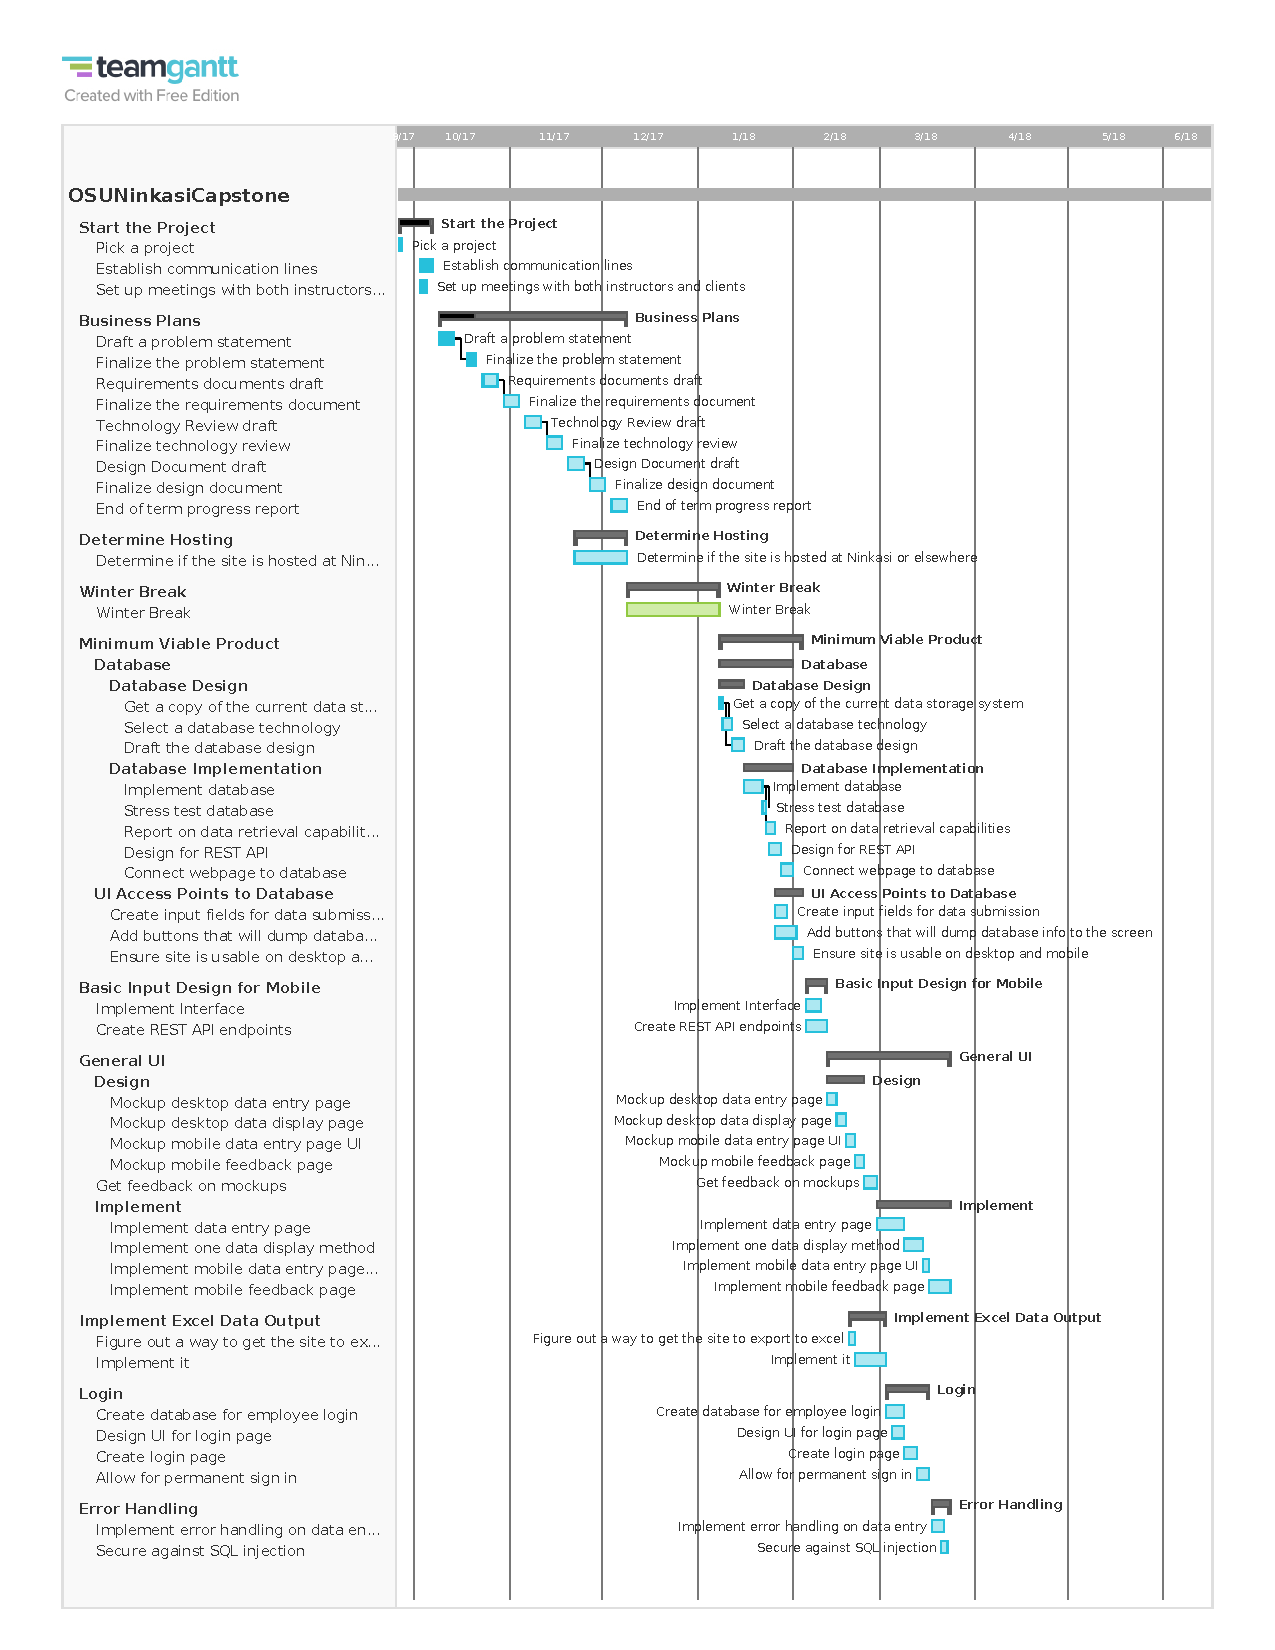
\includepdf[pages=1-2]{OSUNinkasiCapstone.pdf}

\end{document}
